\subsection{Model Architecture Novelties}

We adopt T5 as our core architecture, but additionally optimize training and memory usage by applying three key techniques: \textbf{Dynamic Pruning}, \textbf{LoRA}, and \textbf{QLoRA}.

\subsubsection{Dynamic Pruning}
Large-scale DSI frameworks, especially when operating on extensive datasets like MS-MARCO, can consume considerable memory and runtime. While fixed or static pruning methods reduce computational overhead, they also risk discarding parameters essential to retrieval accuracy.

In response, we propose \textbf{Dynamic Pruning}, a type of \textbf{unstructured pruning} which adaptively prunes weights based on real-time feature-importance scores. Concretely:
\begin{itemize}
    \item \textbf{Feature Scoring:} At each training step, the model computes importance indicators (e.g., from attention distributions) that highlight which features most strongly impact retrieval.
    \item \textbf{Dynamic Cutoffs:} A context-dependent threshold then prunes low-importance features while preserving the most influential parameters. Specifically, weights with the smallest magnitudes (by L1 norm) are set to zero.
    \item \textbf{Iterative Refinement:} Throughout training, the thresholds and importance metrics are continuously updated, balancing the removal of redundant weights with the retention of crucial ones.
\end{itemize}
By removing less critical parameters, unstructured pruning substantially lowers memory and computational demands without degrading retrieval performance. In our experiments, Dynamic Pruning—used alongside Mixed Precision and Gradient Accumulation—shortened training time from over five hours to just 45 minutes for each epoch (considering the whole dataset). 

\subsubsection{LoRA: Parameter-Efficient Fine-Tuning}
Fine-tuning large T5 models from scratch can be expensive in both time and GPU memory. To alleviate this, we decided to employ \textbf{LoRA} (Low-Rank Adaptation). In a nutshell, we have that LoRA \emph{freezes} the original T5 weights and injects small low-rank adapter modules into the attention layers. During training, only these adapter weights are updated—dramatically cutting the total trainable parameter count and thus reducing memory needs and speeding up convergence.

\subsubsection{QLoRA: 4-bit Quantization for T5}
Although LoRA alone is parameter-efficient, large T5 models can still require substantial GPU memory. We decide therefore to also provide for an alternative model version (in addition to the basic one and to the LORA version), to further minimize memory consumption, we apply \textbf{QLoRA}, which additionally quantizes the T5 weights to a \emph{4-bit} format using \textit{bitsandbytes} library. In this setup, the base T5 is compressed into 4-bit precision, while LoRA’s low-rank adapters remain at higher precision for effective fine-tuning. This model, further reduce memory requirements and training overhead without sacrificing retrieval accuracy.

\subsubsection{AdaLoRA}
In addition to the original LoRA approach and its quantized version, we explored \textit{Adaptive LoRA} (AdaLoRA) as introduced by \cite{liu2024aloraallocatinglowrankadaptation}. The fundamental idea behind AdaLoRA is to dynamically adjust the effective rank of the LoRA adapters throughout training. By starting with a higher initial rank (\texttt{init\_r}), the model first gains sufficient capacity to represent the task. After a specified warm-up period, AdaLoRA gradually prunes the less important dimensions in the low-rank matrices, converging to a smaller final rank (\texttt{target\_r}). This rank-reduction process is governed by parameters such as:
\begin{itemize}
    \item \textbf{\texttt{tinit}} and \textbf{\texttt{tfinal}}: defining the interval (in steps) during which the rank adaptation is active;
    \item \textbf{\texttt{deltaT}}: controlling how frequently to update (prune or reallocate) the ranks;
    \item \textbf{\texttt{lora\_alpha}} and \textbf{\texttt{lora\_dropout}}: same scaling and dropout parameters as standard LoRA.
\end{itemize}
The benefit of this method is that we can allocate sufficient capacity at the start of training, and let the model self-regularize to a much smaller final rank, thereby reducing the number of trainable parameters and mitigating overfitting. This is especially useful when dealing with large-scale models or when GPU memory is limited as in our case.

\subsection{ConvLoRA (LoCon)}
Another extension to LoRA that we investigated is \textit{ConvLoRA} \cite{zhong2024convolutionmeetsloraparameter}, sometimes referred to as LoCon. This method adds a lightweight convolutional operation to the LoRA adaptation, originally developed and thought for image-generation models (e.g., Stable Diffusion). In the NLP setting, we introduce a small depthwise convolution layer that operates across the sequence dimension, followed by a low-rank linear mapping. Finally, a scaling factor (\texttt{alpha}) and a residual connection are applied, analogous to standard LoRA.

The motivation behind ConvLoRA is to allow the adapter to capture local token-level patterns more effectively than purely linear low-rank updates. The depthwise convolution can emphasize local features, potentially offering a richer representation. The rank of the linear mapping (\texttt{conv\_lora\_rank}) and the kernel size (\texttt{conv\_kernel\_size}) are hyperparameters that can be tuned. The idea is to freeze all the original transformer parameters and only training the convolutional and low-rank projection weights, preserving most of the benefits of parameter-efficient fine-tuning while enriching the local feature modeling.

% 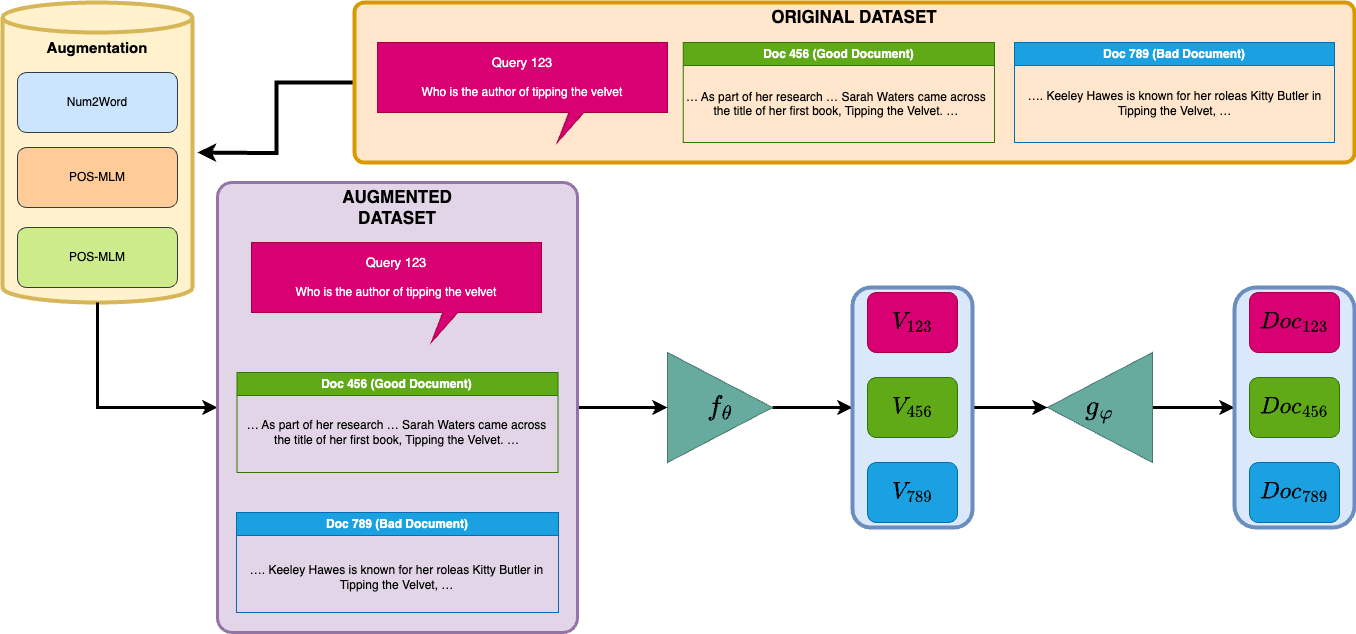
\includegraphics[width=\textwidth]{DS1_1.png}
\subsubsection{Comparison of Techniques}
In summary, we have that Table~\ref{tab:comparison} summarizes the main differences among the proposed methods for memory-efficient fine-tuning and optimization. We highlight key ideas, how each method impacts model parameters and memory usage, and any special advantages or considerations.

\begin{table*}[h]
\centering
\begin{tabular}{p{2.1cm}p{2.8cm}p{3.0cm}p{5.5cm}}
\toprule
\textbf{Technique} & \textbf{Key Idea} & \textbf{Memory/Params Impact} & \textbf{Advantages / Notes} \\
\midrule

\textbf{LoRA} 
& Inserts low-rank adapters in the attention layers
& Very few additional trainable parameters 
& Parameter-efficient fine-tuning; simpler training, fast convergence. \\

\textbf{QLoRA} 
& Quantizes base model to 4-bit and LoRA
& Smaller memory footprint than LoRA 
& Maintains higher-precision adapters for fine-tuning while cutting base-model GPU usage. \\

\textbf{AdaLoRA} 
& Dynamically adjusts the rank of the LoRA adapters 
& Freezes base  and variable-rank adapters 
& Allows higher rank initially for better capacity, then prunes rank to mitigate overfitting.  \\

\textbf{ConvLoRA (LoCon)} 
& Depthwise convolution layer before low-rank projection 
& Small convolution and low-rank adapter 
& Better local token-level pattern modeling than LoRA \\
\bottomrule
\end{tabular}
\caption{\textbf{LoRA Family Comparison} these techniques are used for efficient T5-based DSI fine-tuning.}
\label{tab:comparison}
\end{table*}


